\documentclass[a4paper,11pt]{report}
\usepackage[french]{babel}
\usepackage[T1]{fontenc}
\usepackage[utf8]{inputenc}
\usepackage{lmodern}
\usepackage{microtype}
\usepackage{hyperref}
\usepackage{tabulary}
\usepackage{framed}
\usepackage{fancyhdr}
\usepackage{amsmath}
\usepackage{bbm}
\usepackage{graphicx}
%\usepackage{pst-all}
%\usepackage{xcolor}
%\usepackage{nopageno}

%\newcommand{\latin}[1]{\textit{#1}}

\usepackage[margin=1.0in]{geometry}

%%%%%%%%%%%%%%
%\usepackage{geometry}
 %\geometry{
% a4paper,
 %total={210mm,297mm},
 %left=20mm,
 %right=20mm,
 %top=20mm,
 %bottom=20mm,
 %}
 %%%%%%%%%%%%%%
 
\pagestyle{empty}

\pagestyle{fancy}
\fancyhead{}
\renewcommand{\headrulewidth}{0.5pt}
\fancyhead[R]{\textit{\nouppercase{\rightmark}}}
\fancyfoot{}
\renewcommand{\footrulewidth}{0.5pt}
\fancyfoot[L]{\textit{\nouppercase{\leftmark}}}
\fancyfoot[R]{\thepage}
  
\begin{document}
	\begin{titlepage}
		\vspace*{\stretch{2}}
		\begin{center}
			\large\bfseries\itshape Stage ETE 2015\\
		\end{center}
		\noindent\rule{\linewidth}{3pt}

		\begin{center}
			\Huge\bfseries\itshape Description du système\\
		\end{center}
		
		\noindent\rule{\linewidth}{3pt}
		\begin{center}
			\bfseries
			\large F-PHT \\
			\large Un système d'index de filtres de Bloom pour la recherche d'information par mots clés
		\end{center}
		\vspace*{\stretch{2}}
		\begin{center}
			Réalisé par \textbf{DOAN} Cao Sang \\
			Encadrant: M. \textbf{MAKPANGOU} Mesaac, Regal
		\end{center}
		\vspace*{\stretch{0.5}}
		\begin{center}
			1 Juillet 2015
		\end{center}
	\end{titlepage}

\tableofcontents
\newtheorem{algorithme}{Algorithme}


\chapter{Vue globale}
\section{Prefix Hash Tree (PHT)}
	Un arbre préfixe est un arbre numérique ordonné qui est utilisé pour stocker une table associative où les clés sont généralement des chaînes de caractères. Contrairement à un arbre binaire de recherche, aucun nœud dans le trie ne stocke la chaîne à laquelle il est associé. C'est la position du nœud dans l'arbre qui détermine la chaîne correspondante\footnote{Wikipédia}.
	
	Pour tout nœud, ses descendants ont en commun le même préfixe. La racine est associée à la chaîne vide. Des valeurs ne sont pas attribuées à chaque nœud, mais uniquement aux feuilles et à certains nœuds internes se trouvant à une position qui désigne l'intégralité d'une chaîne correspondante à une clé.
	
	Pour faire une recherche d'une valeur associée à une clé, au départ, on se situe à la racine de l'arbre, en prenant le premier élément de la clé de la requête, on trouve le chemin étiqueté par cet élément, s'il n'existe pas, on est sûr que cette clé n'est pas dans l'arbre. Dès que l'on trouve le chemin, on arrive sur le bon nœud et continue en prenant le deuxième élément de la clé de requête, on applique cette méthode jusqu'à quand on trouve cette clé et se termine sur une feuille.
	
	\begin{figure}[!htbp]
	\centering
	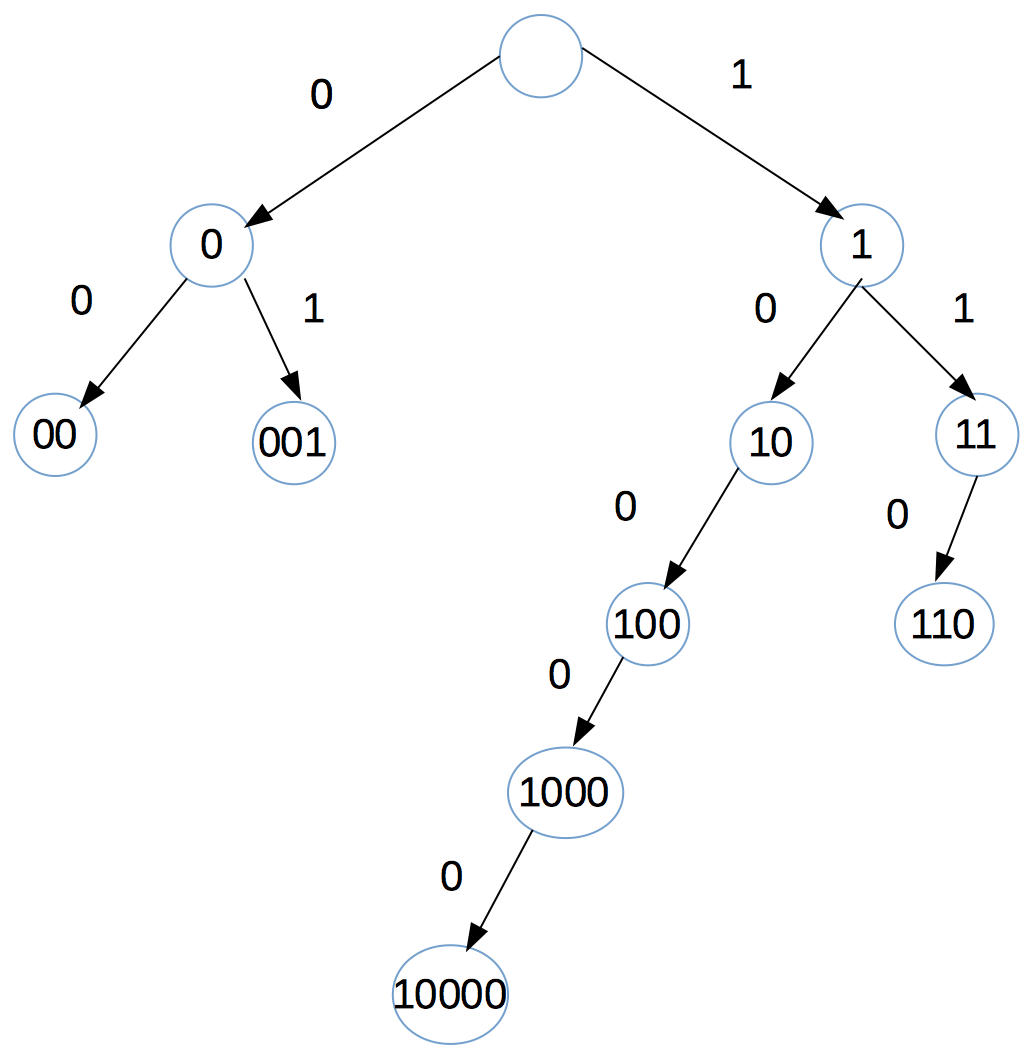
\includegraphics[width=12cm]{PHT.eps}
	\caption{Arbre de préfixe}
	\label{PHT}
	\end{figure}	

\newpage	
	
\section{F-PHT}
	F-PHT est un arbre préfixe de "multibit". Pour stocker une clé, on suit le chemin étiqueté par les fragments successifs de cette clé (dans l'ordre de leur rang) jusqu'à ce qu'on arrive sur une feuille pouvant stocker cette clé.

	Un fragment est un morceau d'une clé (sous-ensemble de bits). Si on considère les clés de taille \textit{m}, le système découpe chaque clé en \textit{f} fragments de taille identique. Par convention, ces fragments sont numérotés de \textit{0} à \textit{f-1}.
	
	\begin{table}[!h]
		\centering		
		\begin{tabular}{|l|*{14}{c|}r|}
		\multicolumn{1}{c}{{\scriptsize 15}} &\multicolumn{1}{c}{}&\multicolumn{1}{c}{}&\multicolumn{1}{c}{}&
		\multicolumn{1}{c}{}&\multicolumn{1}{c}{}&\multicolumn{1}{c}{}&\multicolumn{1}{c}{}&
		\multicolumn{1}{c}{}&\multicolumn{1}{c}{}&\multicolumn{1}{c}{}&\multicolumn{1}{c}{}&
		\multicolumn{1}{c}{}&\multicolumn{1}{c}{}&\multicolumn{1}{c}{}&\multicolumn{1}{c}{{\scriptsize 0}}\\
		\hline
			1 & 0 & 0 & \multicolumn{1}{c||}{0} & 
			1 & 1 & 0 & \multicolumn{1}{c||}{1} & 
			0 & 0 & 0 & \multicolumn{1}{c||}{0} & 
			1 & 0 & 1 & 0 \\
		\hline
		\end{tabular}
		\caption{Exemple le filtre de Bloom}
		\label{fragment/filtredeBloom}
	\end{table}
	
	La table \ref{fragment/filtredeBloom} représente une clé de taille \textit{m = 16} bits, elle est ensuite découpée en \textit{f = 4} fragments. Le premier fragment est la suite de bits \textit{"1000"} qui se trouve les plus à gauche de cette clé. Le dernier est \textit{"1010"}.
	
	\begin{figure}[!htbp]
	\centering
	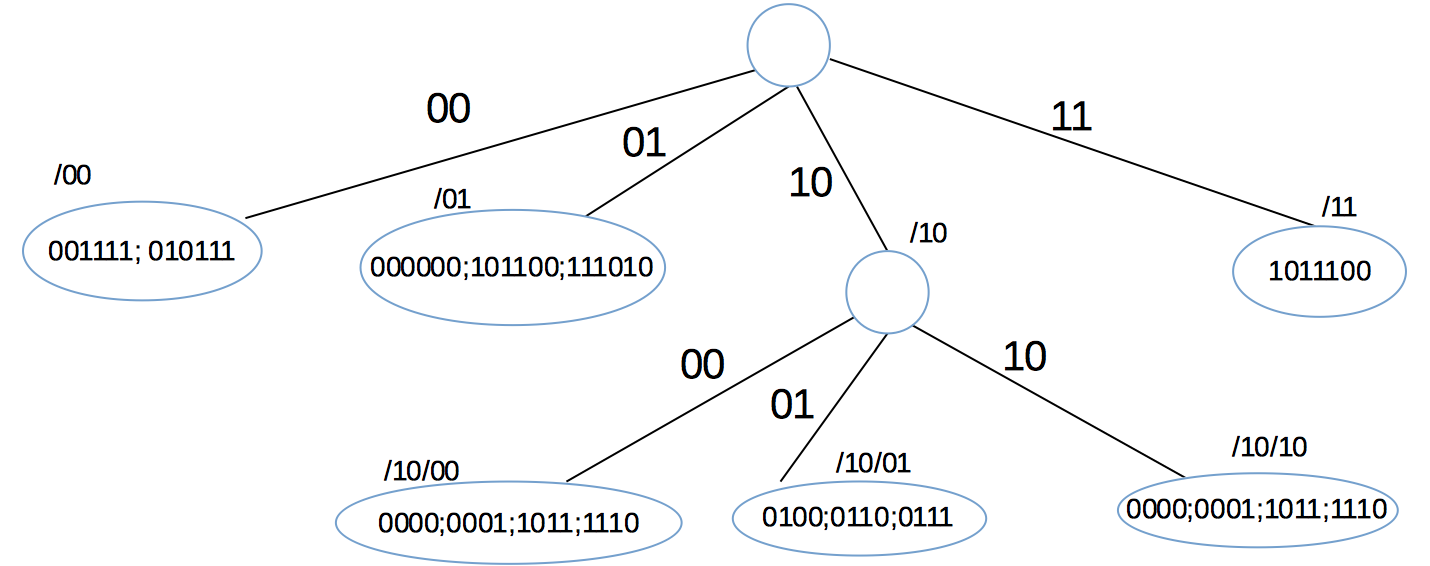
\includegraphics[scale=0.70]{F-PHT_2.eps}
	\caption{Arbre F-PHT}
	\label{F-PHT2}
	\end{figure}	
	
	La figure \ref{F-PHT2} représente l'arbre F-PHT qui stocke une clé de taille \textit{m = 8} bits, la taille d'un fragment est de 2 bits. Au dessus de chaque nœud (interne ou feuille) se trouve son identifiant unique et il caractérise également le chemin unique qui conduit vers ce nœud.
	
\chapter{Système d'indexation}
\section{Objectif}
	Les clés indexées sont des filtres de Bloom de taille \textit{m}.
	L'objectif du système est d'une part de stocker les filtres de Bloom donnés par les utilisateurs, d'autre part de permettre de rechercher tous les filtres de Bloom (stockés dans le système) qui sont sur-ensemble d'un filtre de Bloom caractérisant des mots clés d'une requête.

\section{Architecture du système d'indexation}
	Le système d'indexation est réalisé par un ensemble de serveurs d'index répartis sur plusieurs machines. Chaque serveur gère un ou plusieurs nœuds de l'arbre F-PHT. Ce système permet de créer plusieurs index, chaque index maintient  un F-PHT qui stocke les clés.
	
	On suppose qu'il y a un serveur central connu qui gère tous les index créés. Il utilise une table des index, chaque entrée sert à sauvegarder l'identifiant de l'index \textit{indexID} et le serveur \textit{rootNodeID} qui héberge sa racine. Lorsqu'un utilisateur veut créer/supprimer un index, il demande le serveur central d'ajout/suppression une entrée dans la table des index.

\section{API du système d'indexation}
	Ce système offre aux utilisateurs des services suivants :
	\begin{description}
		\item[	createIndex() 	 :] créer un nouveau index et rend aux l'utilisateur l'identifiant d'index créé \textit{indexID}.
		\item[	removeIndex(indexID)	 :] supprime un index identifié par \textit{indexID}.
		\item[	add(indexID, key) 		 :] ajoute dans l'index identifié par \textit{indexID} une clé \textit{key}.
		\item[	remove(indexID, key)  :] supprime une clé \textit{key} dans l'index identifié par \textit{indexID}.
		\item[	search(indexID, key\_req) 	 :] recherche dans l'index identifié par \textit{indexID} des sur-ensembles qui satisfont la requête \textit{key\_req}.
	\end{description}

	
\chapter{Fonctionnement du système}
\section{Données de chaque nœud dans l'arbre}
	\begin{description}
		\item[Identifiant d'un nœud] caractérise le nœud. Cet identifiant est calculé grâce au chemin vers ce nœud, et ce chemin est unique.
		\item[Niveau d'un nœud (rang)]  est hauteur dans l'arbre F-PHT.
		\item[Table de routage (localRoute)] sert :
			\begin{itemize}
				\item soit à router chaque requête vers le nœud fils responsable de la traiter.
				\item soit à déterminer l'adresse du conteneur local. Ce conteneur stocke au maximum $\gamma$ éléments.
			\end{itemize}
	\end{description}


\section{Protocole}
\subsection{Ajout d'un filtre de Bloom dans F-PHT}
	Lorsqu'un nœud reçoit une requête d'ajout d'un filtre de Bloom (c'est-à-dire d'une clé), il effectue deux actions :
	\begin{enumerate}
		\item Premièrement, il détermine la valeur du fragment numéro \textit{i} de la clé à ajoutée, avec \textit{i} correspondant au niveau de ce nœud dans l'arbre F-PHT.
		\item Une fois le fragment de la clé de rang \textit{i} déterminé, il consulte l'entrée de la table de routage \textit{localRoute} associée à cette valeur. Trois cas sont à distinguer :
		\begin{enumerate}
			\item Si l'entrée est nulle (aucune clé ayant la même valeur pour le fragment de rang \textit{i} a été ajoutée auparavant), le nœud crée un conteneur local, ajoute son adresse dans cette entrée et stocke la clé reçue dans ce conteneur.
			\item Si l'entrée associée à la valeur du fragment de rang \textit{i} contient l'identifiant d'un nœud fils, on transmet la requête vers ce fils.
			\item Si l'entrée contient l'adresse d'un conteneur local, on ajoute la clé reçue dans ce conteneur. Si après ajout, le nombre d'éléments stockés dépasse le seuil fixé, le nœud crée un nœud fils, lui transmet le conteneur, et met à jour l'entrée correspondante l'adresse de son nouveau fils.
		\end{enumerate}
	\end{enumerate}
		
\subsection{Recherche des filtres de Bloom dans F-PHT}
	Lorsqu'un nœud reçoit une requête de recherche des sur-ensembles d'un filtre de Bloom, il effectue les étapes suivantes :
	\begin{enumerate}
		\item D'abord, il détermine la valeur du fragment numéro \textit{i} de la clé de requête, avec \textit{i} correspondant au niveau de ce nœud dans l'arbre F-PHT.
		\item Ensuite, il consulte toutes les entrées de la table de routage \textit{localRoute} contiennent la valeur du fragment déterminée précédente. Pour chaque entrée, il y a 3 cas à traiter :
		\begin{enumerate}
			\item Si l'entrée est nulle (aucune clé contenant cette valeur du fragment de rang \textit{i}), le nœud continue.
			\item Si l'entrée associée à la valeur du fragment de rang \textit{i} contient l'identifiant d'un nœud fils, on transmet la requête vers ce fils.
			\item Si l'entrée contient l'adresse d'un conteneur local, on collecte tous les filtres qui contiennent la requête. L'ensemble des filtres collectés est retourné comme réponse.
		\end{enumerate}
		\item Puis, il attend toutes les réponses des fils auxquels il ont transmis la requête. Une fois, il reçoit toutes les réponses et réunit avec son ensemble des résultats, il transmet le résultat au père.
	\end{enumerate}
	
\subsection{Suppression d'un filtre de Bloom dans F-PHT}
	Les étapes de la suppression d'un filtre de Bloom dans F-PHT effectuées par un nœud sont :
	\begin{enumerate}
		\item Il détermine la valeur du fragment numéro \textit{i} de la clé de requête, avec \textit{i} correspondant au niveau de ce nœud dans l'arbre F-PHT.
		\item Ensuite, il consulte l'entrée de la table de routage \textit{localRoute} associée à cette valeur. Trois cas sont à distinguer :
		\begin{enumerate}
			\item Si l'entrée est null (aucune clé ayant la même valeur pour le frament numéro \textit{i} a été ajoutée auparavant), le nœud rejette la requête.
			\item Si l'entrée associée à la valeur du fragment de rang \textit{i} contient l'identifiant d'un nœud fils, on transmet la requête vers ce fils.
			\item Si l'entrée contient l'adresse d'un conteneur local, on supprime la clé de requête dans ce conteneur. Si après suppression, ce conteneur devient vide, on supprime ce conteneur et cette entrée dans la table \textit{localRoute}. Si cette table devient vide, il notifie le père de la suppression de son fils et demande le système de supprimer ce nœud. Si le père reçoit la notification de son fils, il vide l'entrée où stocke son adresse. En plus, si la table de routage \textit{localRoute} de son père devient aussi vide, il fait la même procédure comme son fils : notifie son père, demande la suppression du système.
		\end{enumerate}
	\end{enumerate}

\chapter{Implémentation du système (Etape 1)}
	Ce système est implémenté en Java.

\section{Plateforme de simulation}
	Cette plateforme est destinée à simuler le système d'indexation. Elle crée un index, ensuite ajoute des données dans cet index. A la fin, une suite de requête de recherche des données est lancée pour tester le fonctionnement du système. Elle peut également simuler la suppression des données dans le système.
		
	L'application interagit avec le système via l'API.
	
\section{Serveur}
	Le serveur s'occupe de la communication entre le client et le système via une interface d'utilisateur. Le client donc peut créer des index, ajouter des filtres, rechercher et supprimer les filtres et les index qui lui appartiennent.
	
	En plus, le serveur est aussi le lieu où on stocke les nœuds du système. Dans le premier temps, il y a un seul serveur qui gère tous les nœuds du système.
	
\section{Implémentation du nœud}
	Les actions principales du nœud sont : ajout d'un filtre, recherche des filtres correspondants à une requête et suppression d'un filtre dans le système.
\subsection{Données de chaque nœud}
	\begin{description}
		\item[Identifiant du nœud (path)] Car le chemin du nœud est unique, donc, nous avons décidé de le considérer comme ID d'un nœud. Ce chemin est une chaîne de caractères.
		\item[Niveau du nœud dans le système (rang)] est hauteur du nœud dans le système.
		\item[Table de routage (localRoute)] est une table d'une dimension, elle contient l'adresse soit d'un conteneur local, soit d'un conteneur à distance, soit aussi du vide. L'index d'ajout des données dans cette table est calculé par le fragment du rang de son nœud.
	\end{description}
	
	En outre, le nœud doit connaître le serveur qui l'héberge.

\subsection{Ajout'd'un filtre dans le nœud}
	L'action d'ajout d'un filtre de Bloom dans un nœud se déroule selon les étapes suivantes : 
	\begin{enumerate}
		\item Il détermine la valeur du fragment de rang \textit{i} du filtre de la requête. Cette valeur est l'index dans la table \textit{localRoute}
		\item Ensuite, il y a 3 cas à distinguer :
			\begin{enumerate}
				\item Si cette entrée est vide, donc, il crée un conteneur local auquel il ajoute ce filtre.
				\item Si cette entrée contient l'adresse d'un nœud fils, ce nœud retourne au système cette adresse.
				\item Si cette entée contient déjà un conteneur local, si ce conteneur a des places disponibles, il l'ajoute. Sinon, il renvoie ce conteneur au système pour que le système puisse créer un nouveau fils correspondant à cette entrée. Le système appelle la méthode \textbf{spilt()} et répond au nœud appelant l'adresse de son nouveau fils. Cette adresse est ajoutée dans sa table \textit{localRoute} en remplaçant le conteneur local précédent.
			\end{enumerate}
\end{enumerate}

\begin{algorithme}
	Ajout d'un filtre de Bloom dans le nœud \textbf{add}
\end{algorithme}

\begin{flushleft}
	\begin{framed}
		\textbf{IN:} BF \textit{bf}\\
		\textbf{OUT:} Object \textit{o}\\
		\noindent\rule{\linewidth}{0.5pt}

		\begin{enumerate}
			\item Fragment \textit{f} $\leftarrow$ \textit{bf}.getFragment(rang)
			\item Object \textit{o} $\leftarrow$ \textit{localRoute}.get(\textit{f})
			\item 
				\begin{tabbing}
					\textbf{if }\= \textit{o} == \textit{null}\\
						\> ContainerLocal \textit{c} $\leftarrow$ new ContainerLocal\\
						\> \textit{c}.add(\textit{bf})\\
						\> \textit{localRoute}.put(\textit{f}, \textit{c})\\
						\> \textbf{return} \textit{null}\\
					\textbf{else}\\
						\> \textbf{return} \textit{o}\\
					\textbf{end} 
				\end{tabbing}
		\end{enumerate}	
	\end{framed}
\end{flushleft}


\subsection{Recherche des filtres dans le nœud}
	Le nœud reçoit la requête sous forme d'un filtre de Bloom : 
	\begin{enumerate}
		\item Comme l'action \textbf{add}, il doit déterminer le fragment de rang \textit{i} de la requête.
		\item Il parcourt toute la table \textit{localRoute} pour trouver tous les entrées non vides qui contiennent le fragment déterminé de la requête :
			\begin{enumerate}
			\item Si l'entrée correspondante contient l'adresse du conteneur local dont il récupère tous les filtres qui contiennent celui de la requête et ajoute dans l'ensemble de résultats.
			\item Si l'entrée correspondante contient l'adresse du  nœud fils, il l'ajoute également dans l'ensemble de résultats.
			\end{enumerate}
	\end{enumerate}		
	
\newpage
\begin{algorithme}
	Recherche des filtres de Bloom dans le nœud \textbf{search}
\end{algorithme}

\begin{flushleft}
	\begin{framed}
		\textbf{IN:} BF \textit{bf}\\
		\textbf{OUT:} Object \textit{o}\\
		\noindent\rule{\linewidth}{0.5pt}

		\begin{enumerate}
			\item Fragment \textit{f} $\leftarrow$ \textit{bf}.getFragment(rang)
			\item Object \textit{o} $\leftarrow$ \textit{null}
			\item Integer i $\leftarrow$ 0
			\item 
				\begin{tabbing}
					\textbf{wh}\=\textbf{ile }\=i $\leq$ \textit{localRoute}.size()\\
						\> Object \textit{tmp} $\leftarrow$ \textit{null}\\
						\> \textbf{if }\= (\textit{f} $\in$ \textit{i}) \&\& ((\textit{tmp } $\leftarrow$ \textit{localRoute}.get(i)) $\neq$ \textit{null})\\
						\> \> \textbf{if }\= \textit{tmp} \textbf{instance of} ContainerLocal\\
						\> \> \> \textbf{wh}\=\textbf{ile }\textit{tmp}.hasNext()\\
						\> \> \> \> BF \textit{bf\_tmp} $\leftarrow$ \textit{tmp}.next()\\
						\> \> \> \> \textbf{if }\= \textit{bf} $\in$ \textit{bf\_tmp}\\
						\> \> \> \> \> \textit{o}.add(\textit{bf\_tmp})\\
						\> \> \> \> \textbf{end}\\ 
						\> \> \> \textbf{end} \\
						\> \> \textbf{else} /* \textit{tmp} \textbf{instance of} String */\\
						\> \> \> \textit{o}.add(\textit{tmp})\\
						\> \> \textbf{end}\\
						\> \textbf{end}\\ 
						\> i++\\
					\textbf{end}
				\end{tabbing}
			\item \textbf{return} \textit{o}
		\end{enumerate}	
	\end{framed}
\end{flushleft}


\subsection{Suppression d'un filtre dans le nœud}
	Lors de la suppression d'un filtre de Bloom dans le nœud, les étapes sont : 
	\begin{enumerate}
		\item D'abord, il détermine la valeur de fragment de rang \textit{i} du filtre de la requête.
		\item Si \textit{localRoute} ne contient pas ce fragment, donc, il n'y a pas ce filtre dans le système.
		\item S'il existe un entrée non vide dans la table \textit{localRoute}, alors : 
		\begin{enumerate}
			\item Si cette entrée contient un conteneur local, alors il supprime le filtre de la requête dans ce conteneur. Si ce conteneur devient vide, il le supprime dans la table \textit{localRoute}. En plus, si cette table devient aussi vide, il renvoie cette table au système pourqu'il puisse supprimer le nœud qui la contient.
			\item Si cette entrée contient l'adresse d'un nœud fils, il renvoie cette adresse au système.
		\end{enumerate}
	\end{enumerate}

\newpage
\begin{algorithme}
	Suppression d'un filtre de Bloom dans le nœud \textbf{remove}
\end{algorithme}

\begin{flushleft}
	\begin{framed}
		\textbf{IN:} BF \textit{bf}\\
		\textbf{OUT:} Object \textit{o}\\
		\noindent\rule{\linewidth}{0.5pt}

		\begin{enumerate}
			\item Fragment \textit{f} $\leftarrow$ \textit{bf}.getFragment(rang)
			\item 
				\begin{tabbing}
					\textbf{if }\= !\textit{localRoute}.contains(\textit{f})\\
						\> \textbf{return} \textit{null}\\
					\textbf{end}
				\end{tabbing}
			\item Object \textit{o} $\leftarrow$ \textit{localRoute}.get(\textit{f})
			\item
				\begin{tabbing}
					\textbf{if }\= \textit{o} \textbf{instance of} ContainerLocal\\
						\> \textit{o}.remove(\textit{bf})\\
						\> \textbf{if }\= \textit{o}.isEmpty()\\
						\> \> \textit{localRoute}.remove(\textit{f})\\
						\> \textbf{end}\\
						\> \textbf{if }\= \textit{localRoute}.isEmpty()\\
						\> \> \textbf{return} \textit{localRoute}\\
						\> \textbf{end}\\
						\> \textbf{return} \textit{null}\\
					\textbf{end}
				\end{tabbing}
			\item \textbf{return} \textit{localRoute}.get(\textit{f}) /*retourne l'adresse de nœud fils*/
		\end{enumerate}	
	\end{framed}
\end{flushleft}

\section{Implémentation du système d'index}
	Le système d'index gère les nœuds. Les actions autorisées pour les utilisateurs sont : ajout d'un filtre de Bloom, recherche des filtres de Bloom et supprime d'un filtre de Bloom. En plus, il existe des actions internes du système comme \textbf{split}.
	
\subsection{Données du système d'index}	
\begin{description}
	\item[Identifiant de l'index (indexID)] est pour distinguer entre plusieurs index différents.
	\item[Identifiant du server (serverID)] est l'identifiant du server qui gère cet index.
	\item[Capacité maximale d'un conteneur local (gamma)] est la taille maximum du conteneur local du système.
	\item[Table de nœuds (listNode)] contient tous les nœuds dans le système.
\end{description}		
	
	
\subsection{Eclatement d'un niveau dans le système}
	Cette méthode est appelée lorsque le conteneur local est plein, elle prend le conteneur local et le nœud père contenant ce conteneur en entrée.
	D'abord, elle crée le nœud qui corresponde au conteneur. Ensuite, pour chaque élément, elle envoie vers ce nouveau nœud en appelant la méthode \textbf{add}. A la fin, elle ajoute l'adresse de ce nouveau nœud dans la table \textit{localRoute} de son père.
	
\newpage
\begin{algorithme}
	Eclatement d'un niveau dans le système \textbf{split}
\end{algorithme}

\begin{flushleft}
	\begin{framed}
		\textbf{IN:} Node \textit{father}, ContainerLocal \textit{c}\\
		\textbf{OUT:} \textit{null}\\
		\noindent\rule{\linewidth}{0.5pt}

		\begin{enumerate}
			\item BF \textit{bf} $\leftarrow$ \textit{c}.get(0)
			\item Fragment \textit{f} $\leftarrow$ \textit{bf}.getFragment(\textit{father}.getRang())
			\item String \textit{path} $\leftarrow$ \textit{father}.getPath() + \textit{"/"} + \textit{f}
			\item Integer \textit{newRang} $\leftarrow$ \textit{father}.getRang() + 1
			\item Node \textit{n} $\leftarrow$ new Node(\textit{null}, \textit{path}, \textit{newRang}, \textit{gamma}) /*ici, serverID $\leftarrow$ \textit{null}*/
			\item \textit{father}.add(\textit{bf}, \textit{path})
			\item \textit{listNode}.put(\textit{path}, \textit{n})
			\item Integer \textit{i} $\leftarrow$ 0
			\item
				\begin{tabbing}
					\textbf{wh}\=\textbf{ile }\=\textit{i} $<$ \textit{c}.size()\\
						\> \textit{n}.add(\textit{c}.get(i))\\
						\> i++\\
					\textbf{end}
				\end{tabbing}									
		\end{enumerate}	
	\end{framed}
\end{flushleft}

	
\subsection{Ajout d'un filtre de Bloom dans le système}
	Lors de la réception d'une demande d'ajout dans le système, il renvoie cette requête vers le nœud racine, c'est-à-dire le nœud de niveau 0. Il y a 3 cas possibles : 
	\begin{enumerate}
		\item La réponse du nœud est son conteneur local, le système appelle la méthode \textbf{split} et il continue à traiter les autres requêtes.
		\item La réponse du nœud est l'identifiant de son fils, le système cherche ce nœud fils et lui renvoie cette requête.
		\item La réponse du nœud ne contient aucun élément, c'est le succès.
	\end{enumerate}
	Le système continue ce procédure jusqu'à quand l'insertion de ce filtre réussit.
	
\begin{algorithme}
	Ajout d'un filtre de Bloom dans le système \textbf{add}
\end{algorithme}

\begin{flushleft}
	\begin{framed}
		\textbf{IN:} BF \textit{bf} \\
		\textbf{OUT:} \textit{null}\\
		\noindent\rule{\linewidth}{0.5pt}

		\begin{enumerate}
			\item Node \textit{n} $\leftarrow$ \textit{listNode}.get(\textit{"/"})
			\item Object \textit{o} $\leftarrow$ \textit{n}.add(\textit{bf})
			\item
				\begin{tabbing}
					\textbf{wh}\=\textbf{ile }\=\textit{o} $\neq$ \textit{null}\\
						\> \textbf{if }\= \textit{o} \textbf{instance of} ContainerLocal\\
						\> \> \textbf{split(}\textit{n}, \textit{o}\textbf{)}\\
						\> \> \textit{o} $\leftarrow$ \textit{null}\\
						\> \textbf{else}\\
						\> \> \textit{n} $\leftarrow$ \textit{listNode}.get(\textit{o})\\
						\> \> \textit{o} $\leftarrow$ \textit{n}.add(\textit{bf})\\
						\> \textbf{end}\\
					\textbf{end}
				\end{tabbing}									
		\end{enumerate}	
	\end{framed}
\end{flushleft}
	
\subsection{Recherche des filtres de Bloom dans le système}
	Pour la recherche des filtres de Bloom qui matchent la requête, le système renvoie la requête au nœud racine et reçoit le résultat à partir de ce nœud. Le nœud répond au système en envoyant un ensemble de données dans lequel il y a 2 types de données possibles : 
	\begin{enumerate}
		\item soit le filtre de Bloom, simplement, le système l'ajoute dans l'ensemble de filtres trouvés.
		\item soit l'identifiant du nœud fils, alors, il doit y envoyer la requête et traiter sa réponse.
		\item soit rien.
	\end{enumerate}
	A la fin, il retourne le résultat complet.

\begin{algorithme}
	Recherche des filtres de Bloom dans le système \textbf{search}
\end{algorithme}

\begin{flushleft}
	\begin{framed}
		\textbf{IN:} BF \textit{bf} \\
		\textbf{OUT:} ArrayList<BF> \textit{resultat}\\
		\noindent\rule{\linewidth}{0.5pt}

		\begin{enumerate}
			\item Node \textit{n} $\leftarrow$ \textit{listNode}.get(\textit{"/"})
			\item ArrayList<Object> \textit{list} $\leftarrow$ \textit{n}.search(\textit{bf})
			\item ArrayList<BF> \textit{resultat} $\leftarrow$ \textit{null}
			\item
				\begin{tabbing}
					\textbf{wh}\=\textbf{ile }\=\textit{list}.hasNext()\\
						\> Object \textit{o} $\leftarrow$ \textit{list}.next()\\
						\> \textbf{if }\= \textit{o} \textbf{instance of} BF\\
						\> \> \textit{resultat}.add(\textit{o})\\
						\> \textbf{else}\\
						\> \> Node \textit{tmp} $\leftarrow$ \textit{listNode}.get(\textit{o})\\
						\> \> \textit{list}.add(\textit{tmp}.search(\textit{bf}))\\
						\> \textbf{end}\\
					\textbf{end}
				\end{tabbing}
			\item \textbf{return} \textit{resultat}									
		\end{enumerate}	
	\end{framed}
\end{flushleft}


\subsection{Suppression d'un filtre de Bloom dans le système}
	La requête de suppression est aussi envoyée au nœud racine. Il y aussi 3 cas à distinguer :
	\begin{enumerate}
		\item Si la réponse est l'identifiant de son nœud fils, le système y renvoie la requête et attend la réponse.
		\item Si la réponse est une table de routage, cela veut dire que cette table est vide après la suppression de son dernier élément. Le système demande son père de supprimer l'entrée correspondante avec le nœud qui gère cette table et supprime ce nœud, si la table de routage de son père devient vide, le système remonte ce procédure vers la racine pour finir la suppression des nœuds vides.
		\item Si la réponse est null, cette méthode finit avec succès.
	\end{enumerate}

\newpage
\begin{algorithme}
	Suppression d'un filtre de Bloom dans le système \textbf{remove}
\end{algorithme}

\begin{flushleft}
	\begin{framed}
		\textbf{IN:} BF \textit{bf} \\
		\textbf{OUT:} \textit{null}\\
		\noindent\rule{\linewidth}{0.5pt}

		\begin{enumerate}
			\item Node \textit{n} $\leftarrow$ \textit{listNode}.get(\textit{"/"})
			\item Object \textit{o} $\leftarrow$ \textit{n}.remove(\textit{bf})
			\item
				\begin{tabbing}
					\textbf{wh}\=\textbf{ile }\textit{o} $\neq$ \textit{null}\\
						\> \textbf{if }\= \textit{o} \textbf{instance of} String /*l'adresse d'un nœud est une chaine de caractères*/\\
						\> \> \textit{n} $\leftarrow$ \textit{listNode}.get(\textit{o})\\
						\> \> \textit{o} $\leftarrow$ \textit{n}.remove(\textit{bf})\\
						\> \textbf{else}\\
						\> \> String \textit{path} $\leftarrow$ \textit{n}.getPath() /*retourne l'adresse de ce nœud*/\\
						\> \> Integer \textit{rang} $\leftarrow$ \textit{n}.getRang()\\
						\> \> \textbf{if }\= \textit{path} == \textit{"/"}\\
						\> \> \> \textbf{return}\\
						\> \> \textbf{end}\\						
						\> \> \textit{listNode}.remove(\textit{path})\\
						\> \> Integer \textit{lastIndex} $\leftarrow$ \textit{path}.lastIndexOf(\textit{"/"}) /*retourne la dernière position de cette caractère*/\\
						\> \> \textit{n} $\leftarrow$ \textit{listNode}.get(\textit{path}.substring(0, \textit{lastIndex}))\\
						\> \> \textbf{wh}\=\textbf{ile }\textit{true}\\
						\> \> \> \textbf{if }\= \textit{n}.remove(\textit{bf}.getFragment(\textit{rang}))\\
						\> \> \> \> \textbf{return}\\
						\> \> \> \textbf{else}\\
						\> \> \> \> \textit{path} $\leftarrow$ \textit{n}.getPath()\\
						\> \> \> \> \textit{rang} $\leftarrow$ \textit{n}.getRang()\\
						\> \> \> \> \textbf{if }\= \textit{path} == \textit{"/"}\\
						\> \> \> \> \> \textbf{return}\\
						\> \> \> \> \textbf{end}\\
						\> \> \> \> \textit{listNode}.remove(\textit{path})\\
						\> \> \> \> \textit{lastIndex} $\leftarrow$ \textit{path}.lastIndexOf(\textit{"/"})\\
						\> \> \> \> \textit{n} $\leftarrow$ \textit{listNode}.get(\textit{path}.substring(0, \textit{lsatIndex}))\\
						\> \> \> \textbf{end}\\
						\> \> \textbf{end}\\
						\> \textbf{end}\\
					\textbf{end}
				\end{tabbing}
		\end{enumerate}	
	\end{framed}
\end{flushleft}

\end{document}









